\expandafter\def\csname CTEX@spaceChar\endcsname{\hspace{1em}}
\documentclass[UTF8, pdftex, notypeinfo, hyperref]{CASthesis}
\usepackage{indentfirst} % 首行缩进
\usepackage{amssymb,bm,mathrsfs,bbm,amscd}
\usepackage{hepunits}
\usepackage{caption,subcaption}
\usepackage{multirow}
\usepackage[hidelinks,bookmarksdepth=4]{hyperref}
\usepackage{xcolor}
\usepackage{listings}
\usepackage{lineno}
\usepackage{pdfpages}
\usepackage[draft]{todonotes}
\usepackage{geometry}
\geometry{left=3.17cm,right=3.17cm,top=2.54cm,bottom=2.54cm}

\setlength{\marginparwidth}{0.5cm}
% 设置图形文件的搜索路径
\graphicspath{{chapter/}{figures/}}

\usepackage{graphicx}          %设置eps转化为pdf
\usepackage{epstopdf}          %插图使用的是eps,生成的是pdf的插图

\usepackage{verbatim}          %可以使用命令注释掉大量的文字

%\usepackage{subfig} 
%\usepackage{subfigure}         %subfigure

% 取消链接的颜色(黑白打印时)
%\hypersetup{
%    colorlinks=false,
%}

% 小节标题靠左对齐
\CTEXsetup[format+={\flushleft}]{section}

\begin{document}


%%%%%%%%%%%%%%%%%%%%%%%%%%%%%%
%% 封面部分
%%%%%%%%%%%%%%%%%%%%%%%%%%%%%%

  % 中文封面内容
  \confidential{}
  \title{BESIII多气隙电阻板室飞行时间探测器刻度方法的研究}
  \author{郭迎晓}
  \advisor{孙胜森~研究员}
  \advisorinstitute{中国科学院高能物理研究所}
  \chinesedegree{硕士}
  \majordegree{工程硕士}
  \major{计算机技术}
  \submitdate{2017~年~6~月}
  \institute{中国科学院高能物理研究所}

  % 英文封面内容
  \englishtitle{Study of calibration of the Multigap-Resistive Plate Chamber as Time of Flight Detector in BESIII experiment}
  \englishauthor{Yingxiao Guo}
  \englishadvisor{Prof. shengsen sun}
  \englishinstitute{Institute of High Energy Physics}
  \englishdegree{Master}
  \englishmajordegree{Engineering}
  \englishdate{June, 2016}

  % 封面
  %\maketitle

  % 英文封面
  %\makeenglishtitle

  \includepdfmerge{cover.pdf, 1-4}
  \includepdfmerge{statement.pdf}                 %直接插入中文,英文的封面

%%%%%%%%%%%%%%%%%%%%%%%%%%%%%%
%% 前言部分
%%%%%%%%%%%%%%%%%%%%%%%%%%%%%%
\frontmatter

  % 摘要
%  % !TeX root = ../main.tex
% !TEX root = ../main.tex
% -*- root: ../main.tex -*-
% -*- program: pdflatex -*-

\begin{abstract}
北京谱仪(BESIII)的物理目标是对~$\tau$-粲(c)物理进行高精度的实验测量并寻找新物理。在较大的动量范围内很好地鉴别区分各种带电粒子是~BESIII~探测器设计的要求。BESIII~探测器的粒子鉴别系统主要由主漂移室(MDC)的~dE/dx~和飞行时间探测器(TOF)组成。飞行时间探测器的主要物理目标是粒子鉴别(PID),粒子鉴别能力的大小由相同动量不同种类粒子的飞行时间差和时间分辨决定。升级改造前的端盖飞行时间探测器采用塑料闪烁体直接耦合光电倍增管的方案,对于~$\pi$~介子,时间分辨达到~138~ps,已经不能满足~BESIII~实验高精度测量的需要。2015~年~10~月,BESIII~实验完成了端盖~TOF~的升级改造,用时间分辨性能更好的多气隙电阻性板室(MRPC)替代了原来的闪烁体,新的探测器参与了~2015-2016~运行取数。对~MRPC~端盖~TOF~离线数据刻度算法进行研究,并开发相关的软件,通过消除原始测量时间随粒子击中位置和过阈时间(Time over Threshold,TOT)的游动,进一步提高粒子鉴别能力,对实现~BESIII~高精度测量的物理目标是十分重要和不可或缺的。

国际上,相对论重离子对撞机(RHIC)上的~STAR~实验和大型强子对撞机(LHC)上的~ALICE~实验都采用了~MRPC~作为飞行时间探测器,结合他们各自的特点,分别采用多次样条插值和多项式拟合方法进行探测器刻度。

MRPC~端盖~TOF~的离线刻度算法软件基于~BESIII~离线数据处理和分析软件平台(BOSS)。利用~BESIII~实验获得的真实数据,通过在线事例分类得到~Bhabha~事例做为刻度样本,对刻度算法进行了研究。研究对测量时间随带电粒子击中读出条位置,过阈时间的变化关系,以及他们之间的关联进行了分析。论文首先利用多次样条插值方法构造刻度算法,对原始测量时间随过阈时间的复杂的依赖关系进行了刻度,研究发现由于信号反射的存在,这种刻度方法的效果并不理想。通过对过阈时间的击中位置依赖关系的分析,揭示了信号在读出条内的反射造成~TOT~多峰的形成机制。然后在构造刻度公式方法中,首先对击中位置进行了刻度,这个过程同时也消除了过阈时间对击中位置的依赖,然后再对时间-幅度的关系进行刻度,收到了良好的效果,单条时间分辨达到~53.5~ps。论文还对刻度公式的适用性问题,以及刻度算法中过阈时间和击中位置的关联性进行了讨论。最后,论文介绍了离线刻度算法软件的实现。

利用~BESIII~获取的~Bhabha~事例样本,对升级改造后的~MRPC~端盖~TOF~的离线数据刻度算法进行了研究,确定了刻度的流程,构造了合理的刻度公式,完成了相关软件的开发。离线刻度的结果优于探测器硬件设计指标,新的刻度算法将会对~BESIII~获得高精度的测量结果产生积极的促进作用。

\keywords{离线刻度,多次样条插值,多气隙电阻性板室,飞行时间探测器,北京谱仪}
\end{abstract}

\begin{englishabstract}
%北京谱仪(BESIII)的物理目标是对tau-粲(c)物理进行高精度的实验测量并寻找新
Physics goal of BESIII are the tau-c physics in experimental measurement with high precision and searching new physics.
%物理。在较大的动量范围内很好地鉴别区分各种带电粒子是BESIII探测器设计的要求。
In a large range of momentum, it is required to identify all species of charged tracks weel in design of BESIII detector.
%BESIII探测器的粒子鉴别系统主要由主漂移室(MDC)的dE/dx和飞行时间探测器
The particle identification system of BESIII detector consists of Main Drift Chamber(MDC) which is providing the measurement of dE/dx and Time of Flight Detector(TOF).
%(TOF)组成。飞行时间探测器的主要物理目标是粒子鉴别(PID),粒子鉴别能力的大小由相同动量不同种类粒子的飞行时间差和时间分辨决定。升级改造前的端盖飞行时间探
The main physical goal of TOF is to implement the Particle Identification(PID), and PID capability is determined by the different values of the time of flight for different species of particles with the same momentum and the time resolution.
%测器采用塑料闪烁体直接耦合光电倍增管的方案,对于pi介子,时间分辨达到138ps,已经不能满足BESIII实验高精度测量的需%要。2015%年10月,BESIII实验完成了端盖TOF的升级改造,用时间分辨性能更好的多气隙电阻性板室(MRPC)替代了原来的闪烁体,新的%探测器参与了2015~2016运行取数。对MRPC端盖TOF离线数据刻度算法进行研
Before the upgrade, the endcap TOF adopted the project using plastic scintillator coupled with photomultiplier tubes(PMT) directly, and the time resolution is 138ps for pions. However, it couldnot satisfied the requirement of the high precision of BESIII experimental measurement. In October, 2015, the upgraded endcap TOF have been completed in BESIII experiment. And the new endcap TOF based on MRPC which has a better time resolution to substitute plastic scintillator. This new detector technology has been participate the physical data taking in the period of the year 2015 to 2016.
%究,通过消除原始测量时间随粒子击中位置和过阈时间(Time over Threshold,TOT)的游动,进一步提高粒子鉴别能力,对实现%BESIII高精度测量的物理目标是十分重要和不可或缺的。
And the study of the offline data calibration algorithm and develop the relevant software for MRPC endcap TOF is eliminate the original measurement of time with the dependence of the particle hit position and the time-walk of Time over Threshold(TOT), this study further improve the capability of PID, and is important and indispensable to reach the physical goal of high precision measurement at BESIII. 

%国际上,相对论重离子对撞机(RHIC)上的STAR实验和大型强子对撞机(LHC)上的ALICE实验都采用了MRPC作为飞行时间探测器,结合%他们各自的特点,分别采用多次样条插值和多项式拟合方法进行探测器刻度。
Both the STAR experiment in RHIC and the ALICE experiment in LHC used MRPC as their TOF detector. And considering their own characters, the offline date are calibrated using spline-fit method and polynomial fitting method.

%MRPC端盖TOF的离线刻度算法基于BESIII离线数据处理和分析软件平台(BOSS)。利用BESIII实验获得的真实数据,通过在线事例分类得%到Bhabha事例做为刻度样本,对刻度算法进行了研究。
The offline data calibration algorithm of MRPC endcap TOF is based on BESIII offline data processing and analysis software(BOSS). The calibration data sample is Bhabha events of real data which is selected.
%研究对测量时间随带电粒子击中读出条位置,过阈时间的变化关系,以及他们之间的关联进行了分析。论文首先利用多次样条插值方法构造刻度算法,对原始测量时间随过阈时间的复杂的依赖关系进行了刻度,研究发现由于信号反射的存在,这种刻度方法的效果并不理想。通过对过阈时间的击中位置依赖关系的分析,揭示了信号在读出条内的反射造成TOT多峰的形成机制。在构造刻度公式方法中,首先对击中位置进行了刻度,这个过程同时也消除了过阈时间对击中位置的依赖,然后再对时间-幅度的关系进行刻度,收到了良好的效果,时间分辨达到**ps。论文还对刻度公式的适用性问题,以及刻度算法中过阈时间和击中位置的关联性进行了讨论。
This study analyzed the alternative relations of the measurement time changes with hitted positions and TOT of signal, and also  analyzed their the corelation between these variables. This paper first constructed a calibration algorithm by spline-fit method, and calibrated the original measurement time with the complex change of TOT. The Spline fit method is not ideal due to the presence of signal reflections found by studies. Then, the dependency of the hit position of TOT has been investigated, it explained how the reflection of the signal within the readout strips causes the formation mechanism of the TOT multimodal. In the construction of the calibration formula, the hit position has been performed first, at the same time, the hit position dependency of TOT can be eliminated. And then, correct time versus TOT, it has good effect, the time resolution reached 53.5ps in one strip. The applicability of these calibration formula and the relevance between TOT and hit position in calibration algorithm are also discussed in this paper.Finally, the paper introduces the implementation of the software of the offline calibration algorithm.    

%利用BESIII获取的Bhabha事例样本,对升级改造后的MRPC端盖TOF的离线数据刻度算法进行了研究,确定了刻度的流程,构造了合理的刻度公式。离线刻度的结果优于探测器硬件设计指标,新的刻度算法将会对BESIII获得高精度的测量结果产生积极的促进作用。
Using the Bhabha samples collected from BESIII, the offline data calibration algorithm of the upgraded MRPC endcap TOF detector has been studied, determined the process of calibration, constructed reasonable calibration formula and complete the development of relevant software. The result of offline data calibration is better than design target of the detector hardware, and the new calibration algorithm will play a positive role in getting the high precision measurement results at BESIII.


\englishkeywords{Offline Data Calibration,Spline Fit,Multi-gap Resistive Plate Chamber, Time of Flight Counter,BESIII}

\end{englishabstract}


  % 目录
  \tableofcontents
  % 表格目录
  \listoftables
  % 插图目录
  \listoffigures


%%%%%%%%%%%%%%%%%%%%%%%%%%%%%%
%% 正文部分
%%%%%%%%%%%%%%%%%%%%%%%%%%%%%%
\mainmatter

%  \include{chapter/}
%  % !TeX root = ../main.tex
% !TEX root = ../main.tex
% -*- root: ../main.tex -*-
% -*- program: pdflatex -*-
\chapter{利用样条插值方法对~MRPC~进行刻度}

~MRPC-TOF~直接测量的信息包括原始的飞行时间和过阈时间(~time-over-threshold~,简称~TOT~)。为了得到精确的飞行时间信息,还需要对时幅游走、过大信号、粒子在对数条上的传播时间,以及在电子学电缆等的时间延迟等因素进行刻度和修正,还要进行离线分析。为了得到良好的时间分辨,必须对不同粒子的样本进行离线的刻度和修正,得到相应的刻度常数,再对原始数据进行重建从而得到飞行时间探测器的性能。
%\begin{comment}
~MRPC-TOF~的离线刻度是通过比较测量时间~$t_{mea}=t_{raw}-t_{0}-t_{cor}$~与带电粒子从对撞顶点到击中~MRPC-TOF~的预期飞行时间~$t_{exp}=L/\beta c$~来比较,其中~$t_{0}$~是事例的起始时间,~$t_{cor}$~是时间的修正项;~c~是真空中的光
速,$\beta=p/\sqrt{p^2+m^2}$是带电粒子的飞行时间,~m~是粒子的质量,飞行长度~L~和动量~P~是通过主漂移室(~MDC~)测量得到的。飞行时间修正项~$t_{cor}$~是过阈时间~TOT~和~Z~向击中位置的函数。
%\end{comment}
对于每一个读数条,每个读出单元定义:
%\begin{equation}
\begin{displaymath}
\chi^2(counter,readout)=\sum\limits_{event}(t_{mea}-t_{exp})^2
\end{displaymath}
%\end{equation}
通过分析大量的事例样本,进行反复迭代,利用最小~$\chi^2$~方法,刻度常数项可以通过~$\partial\chi^2/\partial P_{i}=0$~得到。在重建中,利用刻度得到的刻度常数对原始的飞行时间信息进行重建,就可以得到经过刻度修正得到的飞行时间信息。

STAR~实验MRPC采用的是样条插值(~spline Fit~)刻度的方法。因此本文也对~BESIII~的~MRPC~进行了样条插值方法的研究。
本章主要介绍样条插值方法。分两部分介绍:先对~TOT~进行插值,之后对击中位置~Z~修正;先对击中位置~Z~进行修正,之后对~TOT~进行插值。并进行了一定的结果比较,发现先修正~Z~,然后对~TOT~进行插值的结果比另一种方法好。

样条插值方法优点:光滑性好,且低阶就能拟合的很好。高能所集群下的~root~中有关于~TSpline~的类包,可以利用它完成样条插值的拟合。

本章数据选用的是~160524-160530~这期间~BESIII~对撞数据中的~Bhabha~事例。选用~Bhabha~事例是因为它事例量大,易于挑选,纯度高,适合做刻度样本。

%%%%%%%%%%%%%%%%%%%%%%%%%%%%%%%%%%%%%%%%%%%%%%%%%%%%%%%%%%%%%%%%%%%%%%%%%%%%%%
\section{修正~Z~前进行插值}
%%%%%%%%%%%%%%%%%%%%%%%%%%%%%%%%%%%%%%%%%%%%%%%%%%%%%%%%%%%%%%%%%%%%%%%%%%%%%%

本节以挑选的~Bhabha~事例中击中位置在~MRPC~中模块编号为~55~,对数条编号为~7~这一个对数条为例。具体做法,就是先对~TOT~进行插值修正,之后对得到的结果再次对~Z~进行修正得到最终的时间分辨等刻度信息。
\subsection{等事例数分~bin~拟合}
\begin{itemize}
    \item 以TOT的大小为度量对所选的事例数进行等事例数分~bin~
    \item 对于每个~bin~区间,进行拟合
    \item 对于上一步得到的~mean~值进行插值,得到插值的刻度常数
    \item 利用上一步得到的刻度常数,对时间信息进行修正 
\end{itemize}
等事例数分~bin~的原因是时间随~TOT~的分布是不均匀的。在小~q~(声明:以下所有出现~q~都等同于~TOT~)和大~q~部分事例数很少,如果采用等区间分~bin~的话,会出现比较大的误差棒。分~bin~完成后,发现一个~bin~内时间有两个峰值。图~\ref{fig:ScatterDiagram}~是时间对~TOT~的分布,图~\ref{fig:cutScatterDiagram}~是图~\ref{fig:ScatterDiagram}~截取的一部分。

\begin{figure}[htbp]
\begin{minipage}[t]{0.5\linewidth}
%\centering
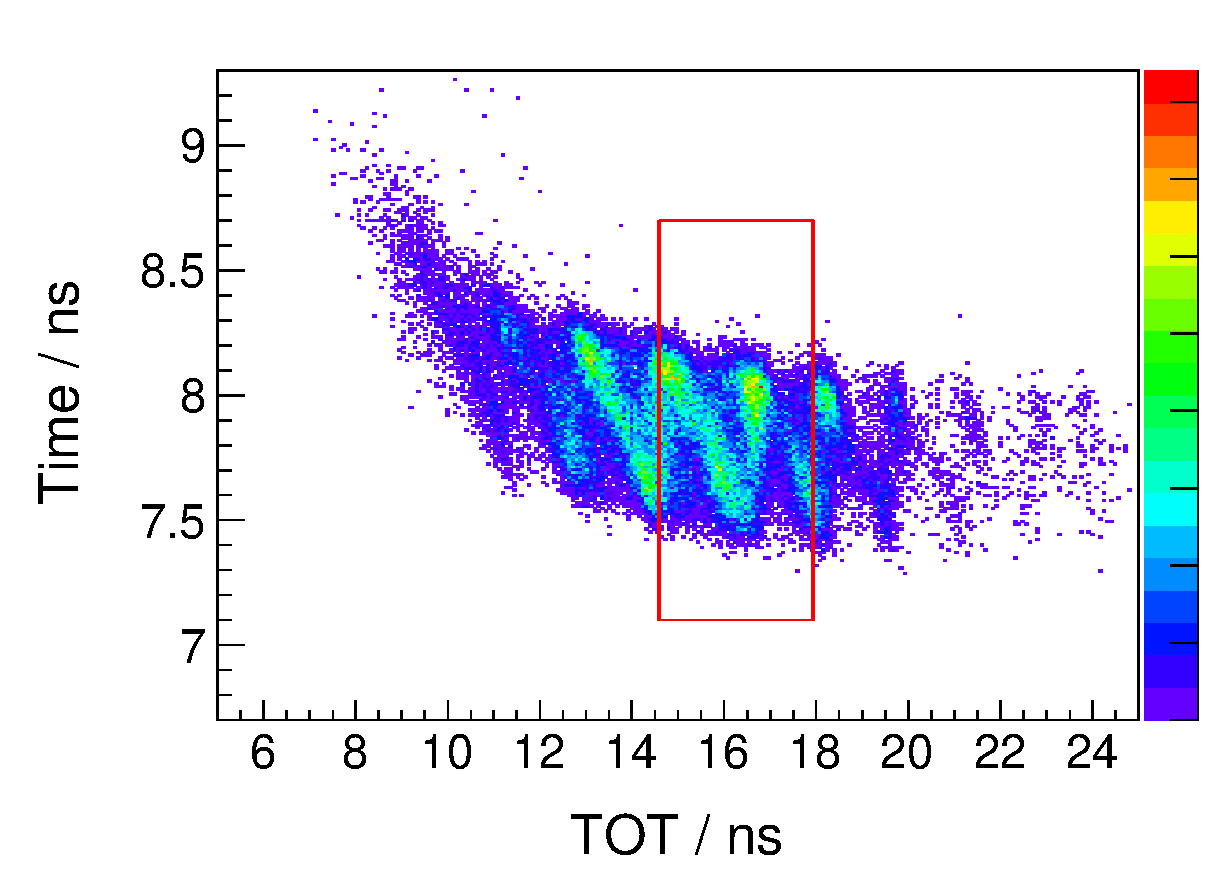
\includegraphics[width=0.9\textwidth]{chap2/ScatterDiagram.eps}
\subcaption{时间对TOT的分布}
\label{fig:ScatterDiagram}
\end{minipage}%
\hfill
\begin{minipage}[t]{0.5\linewidth}
%\centering
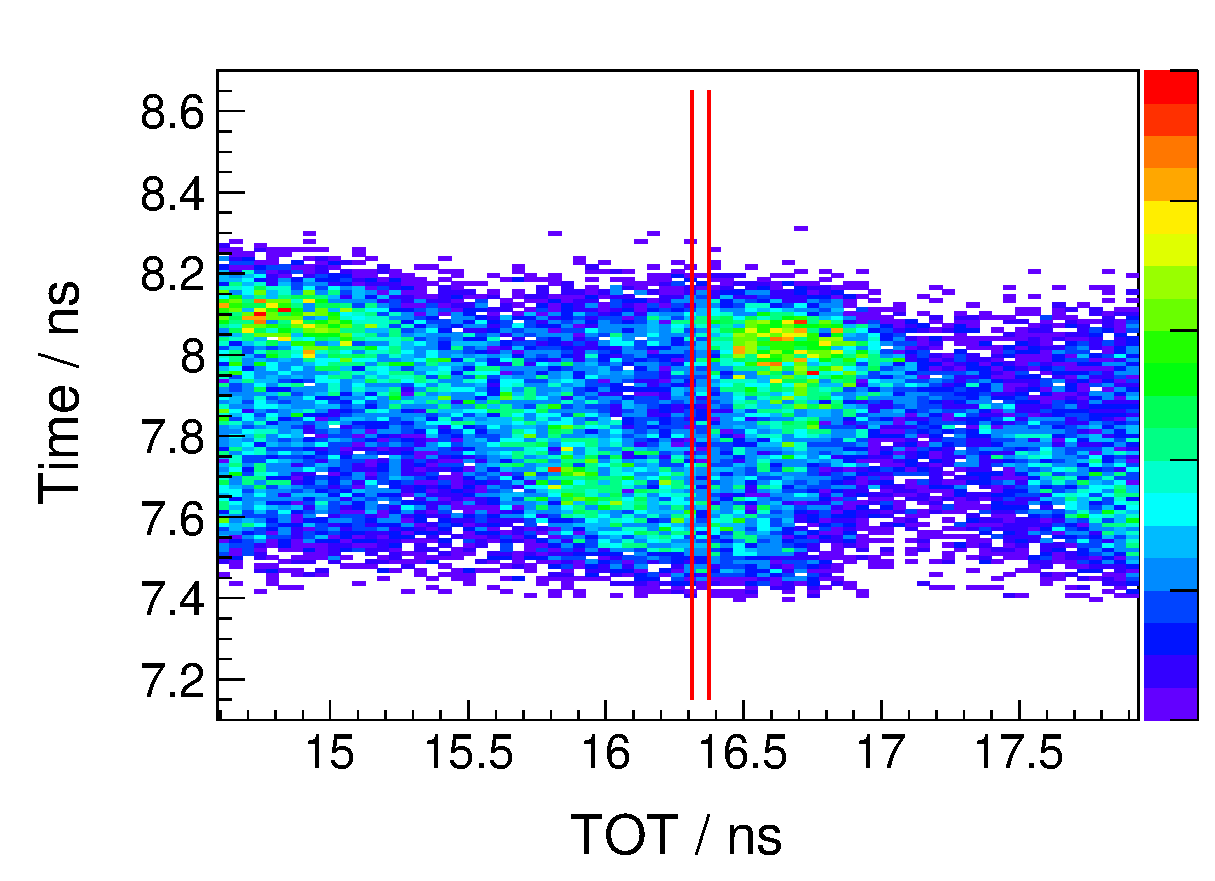
\includegraphics[width=0.9\textwidth]{chap2/cutScatterDiagram.eps}
\subcaption{截取时间对TOT的分布}
\label{fig:cutScatterDiagram}
\end{minipage}
\caption{时间对TOT的分布}
%\label{fig:Diagram}
\end{figure}

\begin{figure}[htbp]
\centering
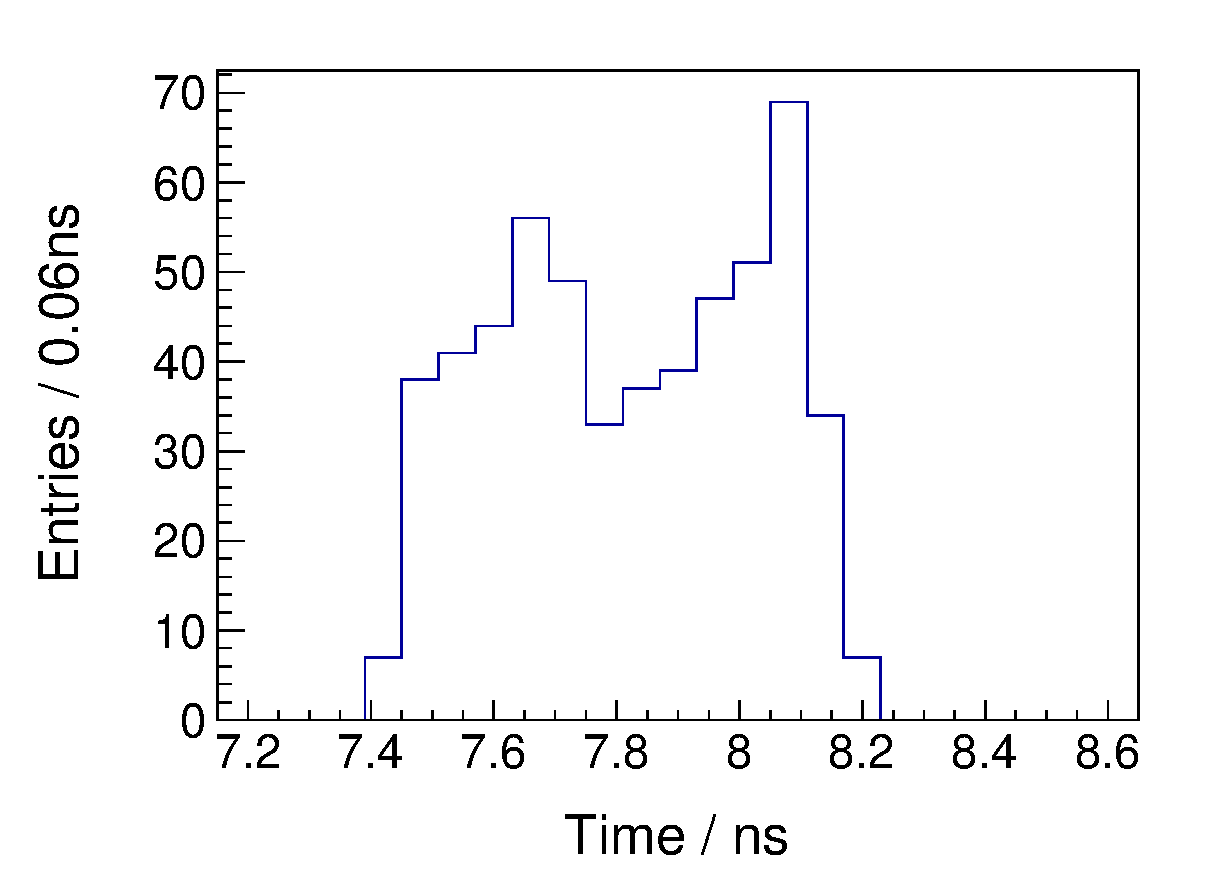
\includegraphics[width=0.5\textwidth]{chap2/onebinTime.eps}
\caption{截取一个bin的时间分布}
\label{fig:onebinTime}
\end{figure}

图~\ref{fig:onebinTime}~是一个bin内的时间分布,可以明显看出具有双峰。对此,我没有办法在一个区间内得到一个合适的中心值。

\subsection{两个高斯拟合和单个高斯拟合}

图~\ref{fig:double-ScatterDiagram}~,~\ref{fig:single-ScatterDiagram}~分布是对每个~bin~用两个高斯和一个高斯函数拟合后得到的中心值的分布

\begin{figure}[!h]
\begin{minipage}[!h]{0.5\linewidth}
%\centering
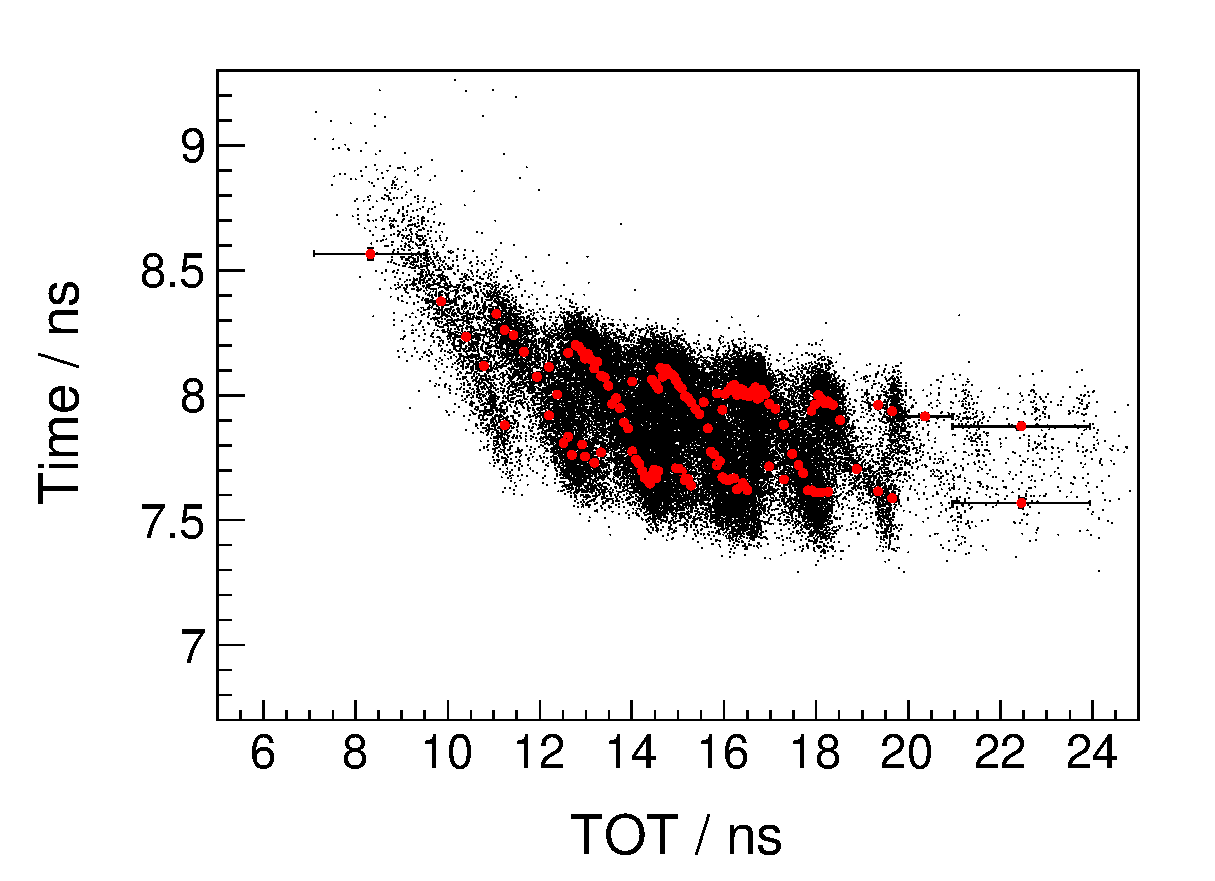
\includegraphics[width=0.95\textwidth]{chap2/double-ScatterDiagram.eps}
\subcaption{两个高斯拟合后的graph}
\label{fig:double-ScatterDiagram}
\end{minipage}%
\hfill
\begin{minipage}[!h]{0.5\linewidth}
%\centering
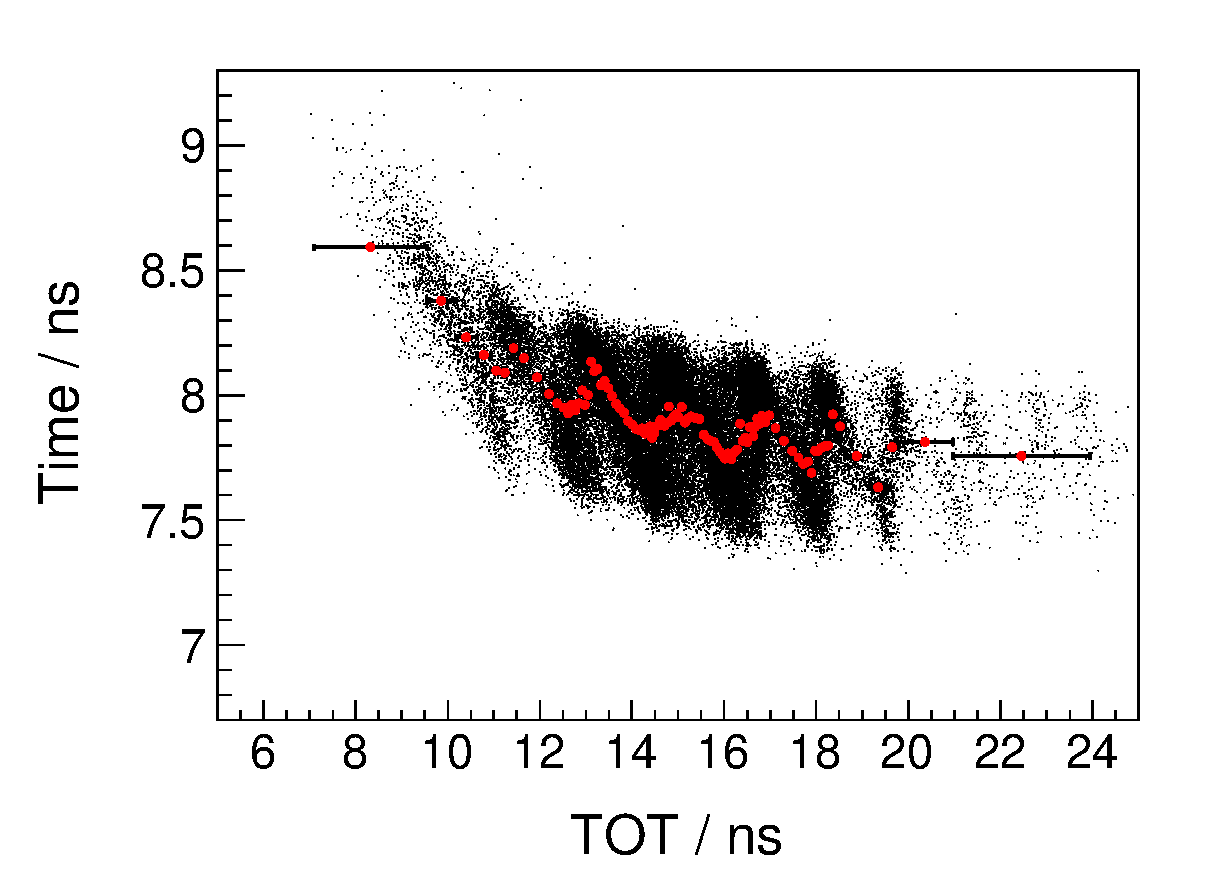
\includegraphics[width=0.95\textwidth]{chap2/single-ScatterDiagram.eps}
\subcaption{一个高斯拟合后的graph图}
\label{fig:single-ScatterDiagram}
\end{minipage}
\caption{高斯拟合后的graph}
\end{figure}

图~\ref{fig:double-leftspline}~第一种做法的样条插值曲线,每个~bin~的时间的中心值取那个比例高的。图~\ref{fig:single-leftspline}~第二种做法的样条插值曲线。可以看出,样条曲线已经把之前graph点的趋势拟合了。

\begin{figure}[!h]
\begin{minipage}[!h]{0.5\linewidth}
%\centering
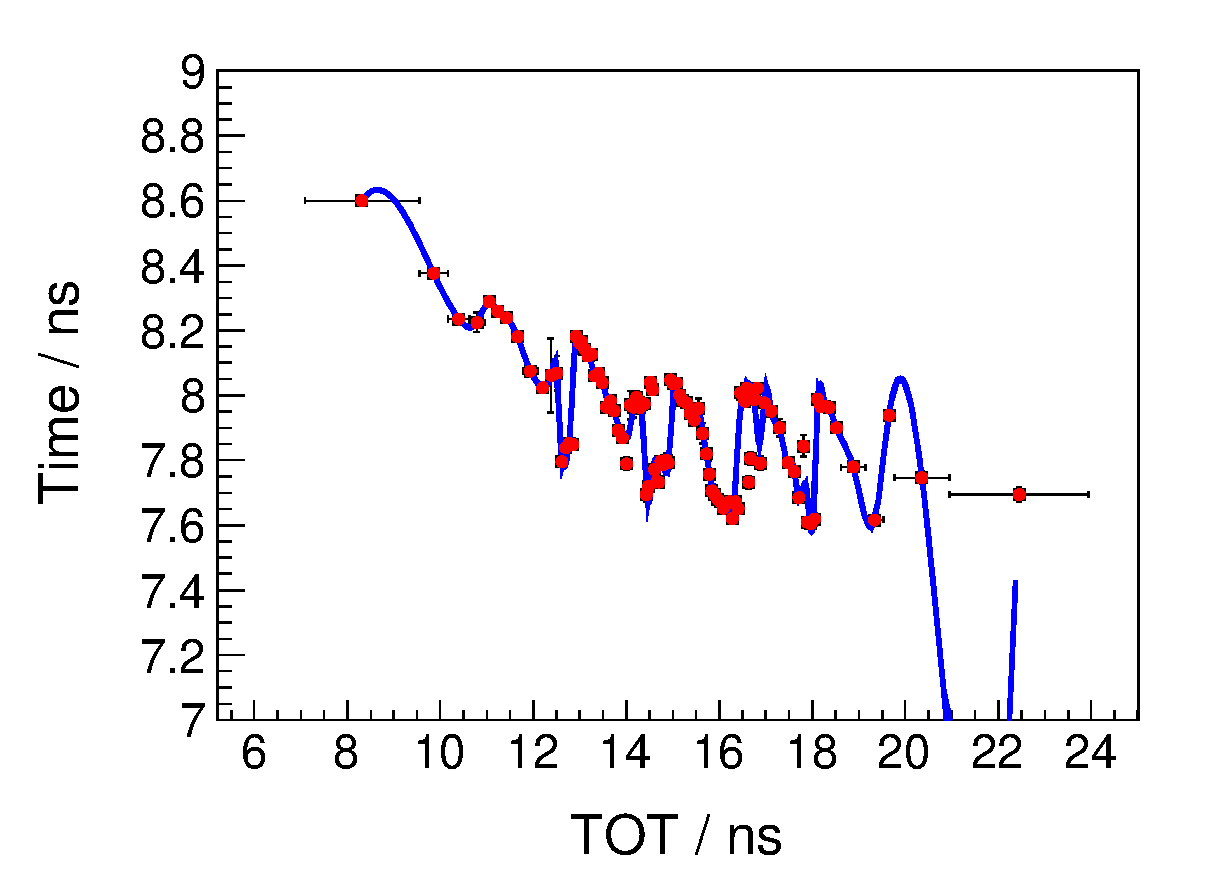
\includegraphics[width=0.95\textwidth]{chap2/double-leftspline.eps}
\subcaption{两个高斯拟合得到的中心值的样条插值}
\label{fig:double-leftspline}
\end{minipage}%
\hfill
\begin{minipage}[!h]{0.5\linewidth}
%\centering
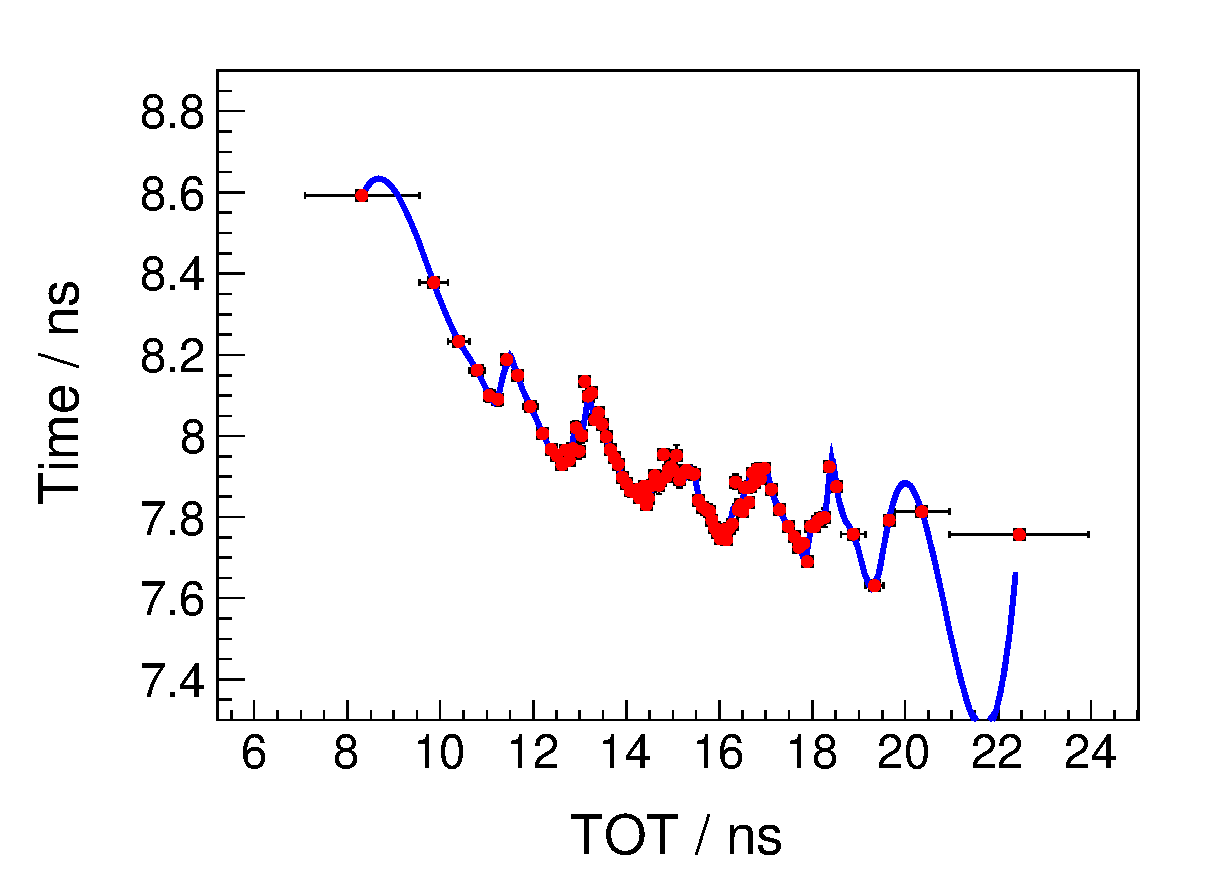
\includegraphics[width=0.95\textwidth]{chap2/single-leftspline.eps}
\subcaption{一个高斯拟合得到的中心值的样条插值}
\label{fig:single-leftspline}
\end{minipage}
\caption{样条插值}
\end{figure}

\subsection{~Z~的修正}
不管上述的哪种方法,插值修正完~TOT~后,时间随~Z~的分布都还有依赖,对此进行一个~Z~项的修正,然后得到时间分辨。图~\ref{fig:double-leftspline}~第一种做法得到的时间分辨,为~160ps~;图~\ref{fig:single-leftspline}~第二种做法得到的时间分辨,为~92ps~。这个结果和下一节先修正~Z~,后修正~TOT~的结果相比,差别很大。

分析原因:~TOT~的多峰来自反射。一次反射内,时间对~TOT~的依赖近似线性关系,样条插值的光滑性决定不能完全描述这种关系。
\begin{figure}[!h]
\begin{minipage}[!h]{0.5\linewidth}
%\centering
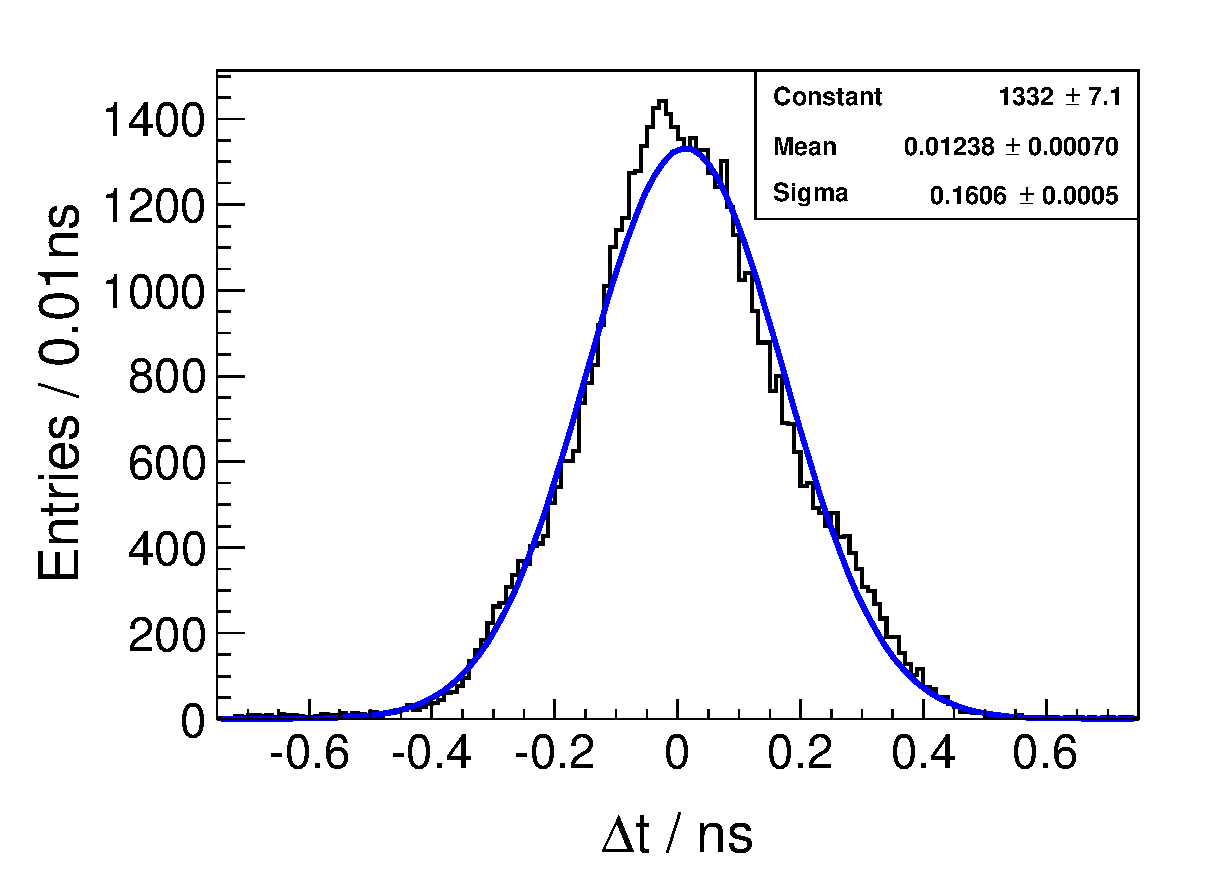
\includegraphics[width=0.8\textwidth]{chap2/double-resolutiongauss.eps}
\subcaption{时间分辨1}
\label{fig:double-resolutiongauss}
\end{minipage}%
\hfill
\begin{minipage}[!h]{0.5\linewidth}
%\centering
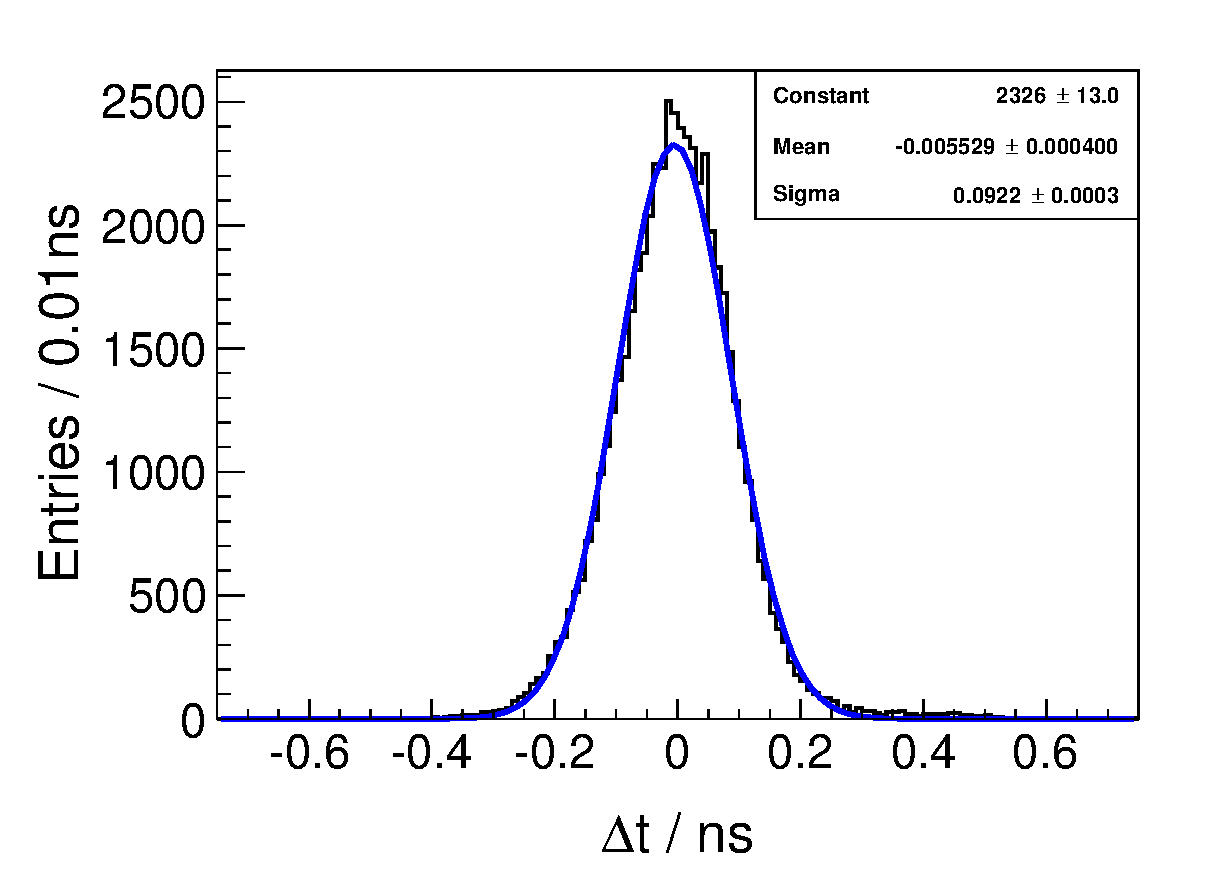
\includegraphics[width=0.8\textwidth]{chap2/single-resolutiongauss.eps}
\subcaption{时间分辨2}
\label{fig:single-resolutiongauss}
\end{minipage}
\caption{时间分辨}
\end{figure}

\subsection{反射问题}


图~\ref{fig:TOT}~是信号的过阈时间。对于一定的阈值,幅度大小不同的信号,对应的过阈时间不同。信号幅度越大,过阈时间也就越大。
图~\ref{fig:reflection}~是~MRPC~读数条的反射问题,分为近端反射和远端反射。由于读数条本身较短,反射信号只是比真实信号时间晚不到1ns,这样导致反射信号和原来的真实信号叠加。测量的~TOT~也就变大了。
正是由于过阈时间和反射问题的存在,导致时间对~TOT~的分布复杂。对时间和~TOT~的关系的研究也刻度研究的重点和难点部分。

\begin{figure}[!h]
\begin{minipage}[!h]{0.5\linewidth}
%\centering
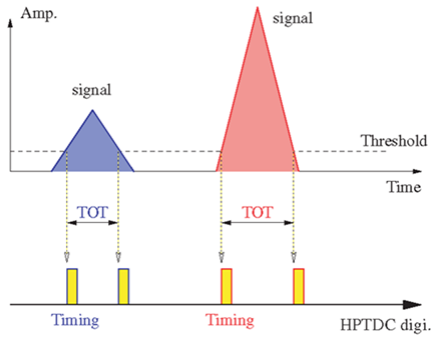
\includegraphics[width=0.8\textwidth]{chap2/TOT.png}
\subcaption{过阈时间~\cite{Shao:2009aa}~}
\label{fig:TOT}
\end{minipage}
\hfill
\begin{minipage}[!h]{0.5\linewidth}
%\centering
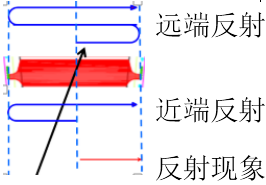
\includegraphics[width=0.9\textwidth]{chap2/reflection.png}
\subcaption{反射问题}
\label{fig:reflection}
\end{minipage}%
\caption{反射问题和过阈时间}
\end{figure}


%%%%%%%%%%%%%%%%%%%%%%%%%%%%%%%%%%%%%%%%%%%%%%%%%%%%%%%%%%%%%%%%%%%%%%%%%%%%%%%
\section{修正~Z~后进行插值}
%%%%%%%%%%%%%%%%%%%%%%%%%%%%%%%%%%%%%%%%%%%%%%%%%%%%%%%%%%%%%%%%%%%%%%%%%%%%%%

\subsection{~Z~向的修正后,时间对~TOT~的分布}

图~\ref{fig:q-before}~和图~\ref{fig:q-after}~是~Z~修正前后时间对~TOT~的分布。可以看出,修正完~Z~后时间对~TOT~的折线几乎消失。在此基础上,对~TOT~进行插值拟合。
\begin{figure}[!h]
\begin{minipage}[!h]{0.5\linewidth}
%\centering
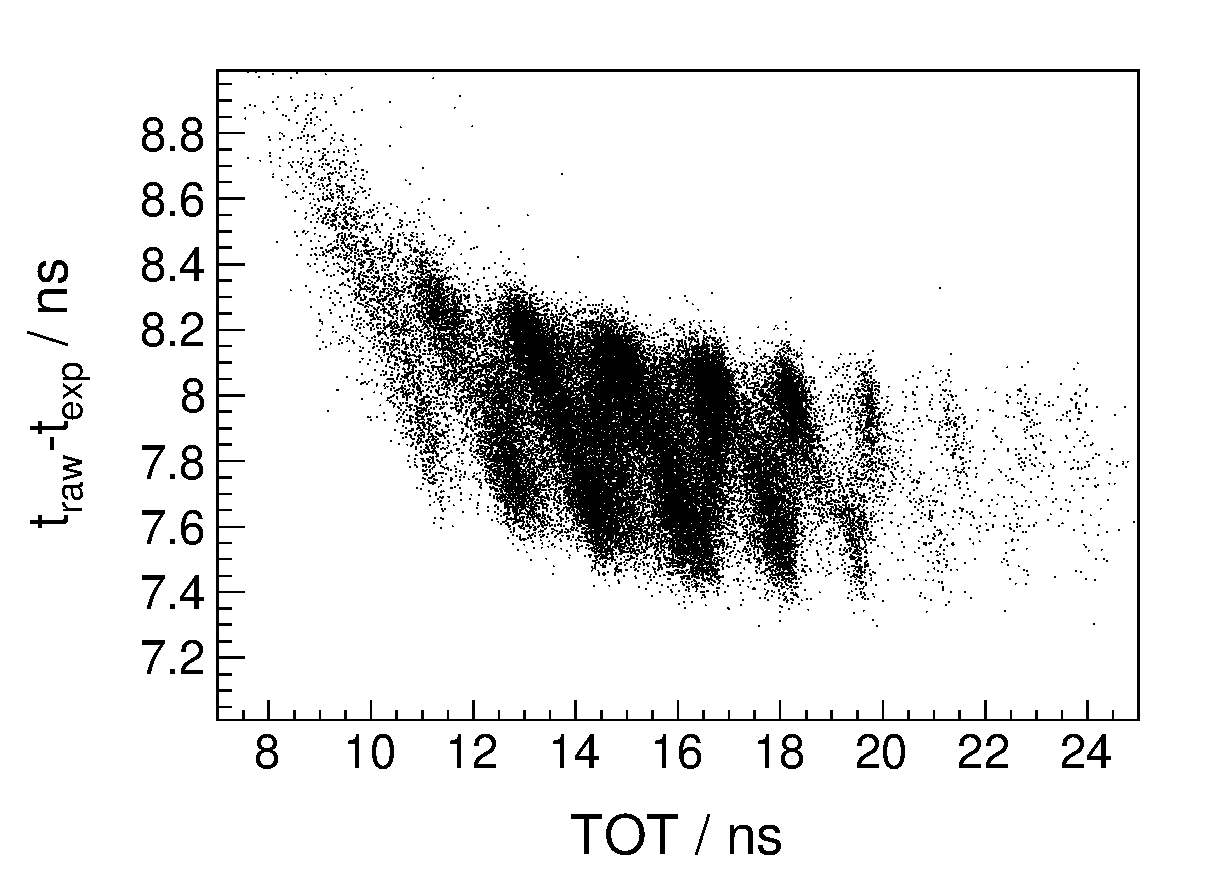
\includegraphics[width=0.9\textwidth]{chap2/q-before.eps}
\subcaption{~Z~修正前}
\label{fig:q-before}
\end{minipage}%
\hfill
\begin{minipage}[!h]{0.5\linewidth}
%\centering
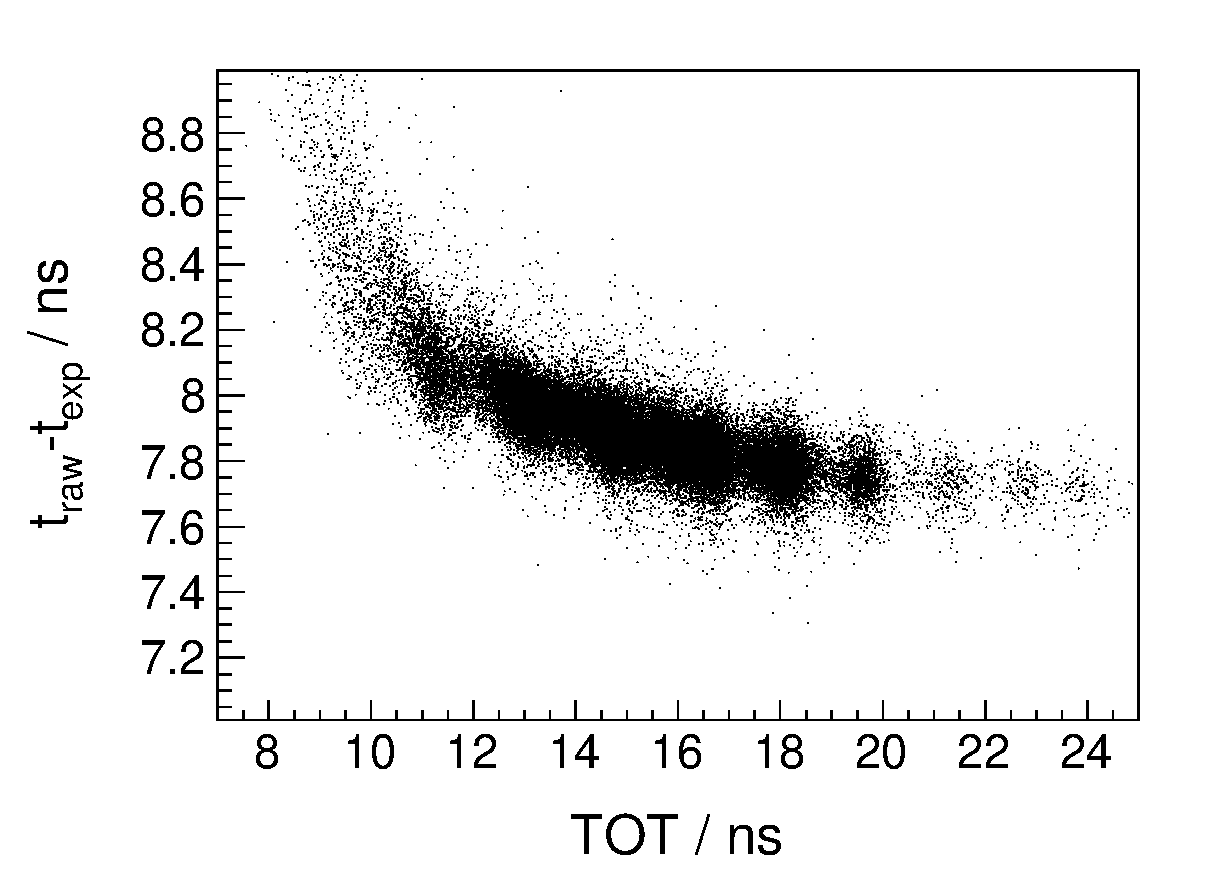
\includegraphics[width=0.9\textwidth]{chap2/q-after.eps}
\subcaption{~Z~修正后}
\label{fig:q-after}
\end{minipage}
\caption{~Z~修正前后时间对~TOT~的分布}
\end{figure}

\subsection{插值}

图~\ref{fig:after-left-spline}~是修正完~Z~后对~TOT~的样条插值曲线;图~\ref{fig:resolutiongauss}~是这种方法得到的最终的时间分辨,为~64ps~,比之前先对~TOT~插值修正得到的时间分辨好。
\begin{figure}[!h]
\begin{minipage}[!h]{0.5\linewidth}
%\centering
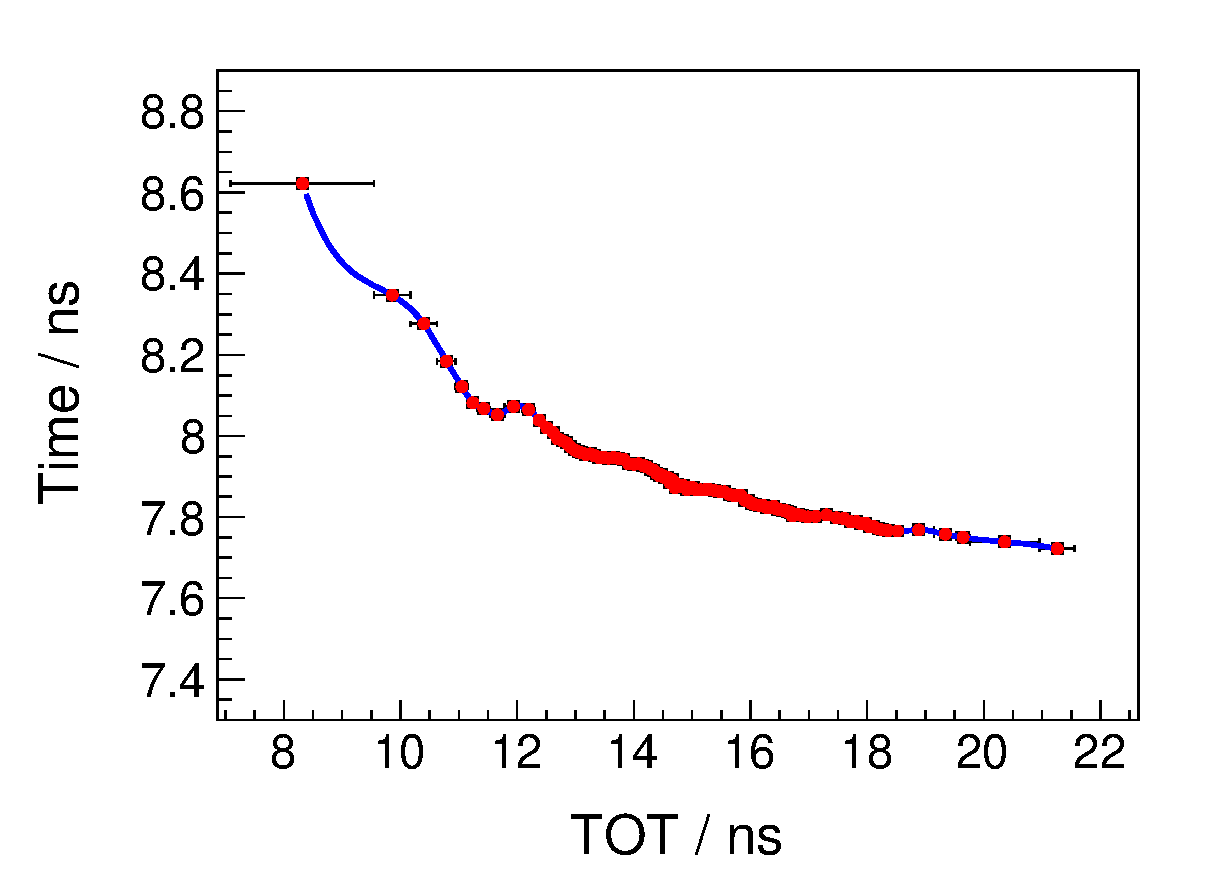
\includegraphics[width=0.9\textwidth]{chap2/after-left-spline.eps}
\subcaption{~Z~修正后对~TOT~进行插值}
\label{fig:after-left-spline}
\end{minipage}%
\hfill
\begin{minipage}[!h]{0.5\linewidth}
%\centering
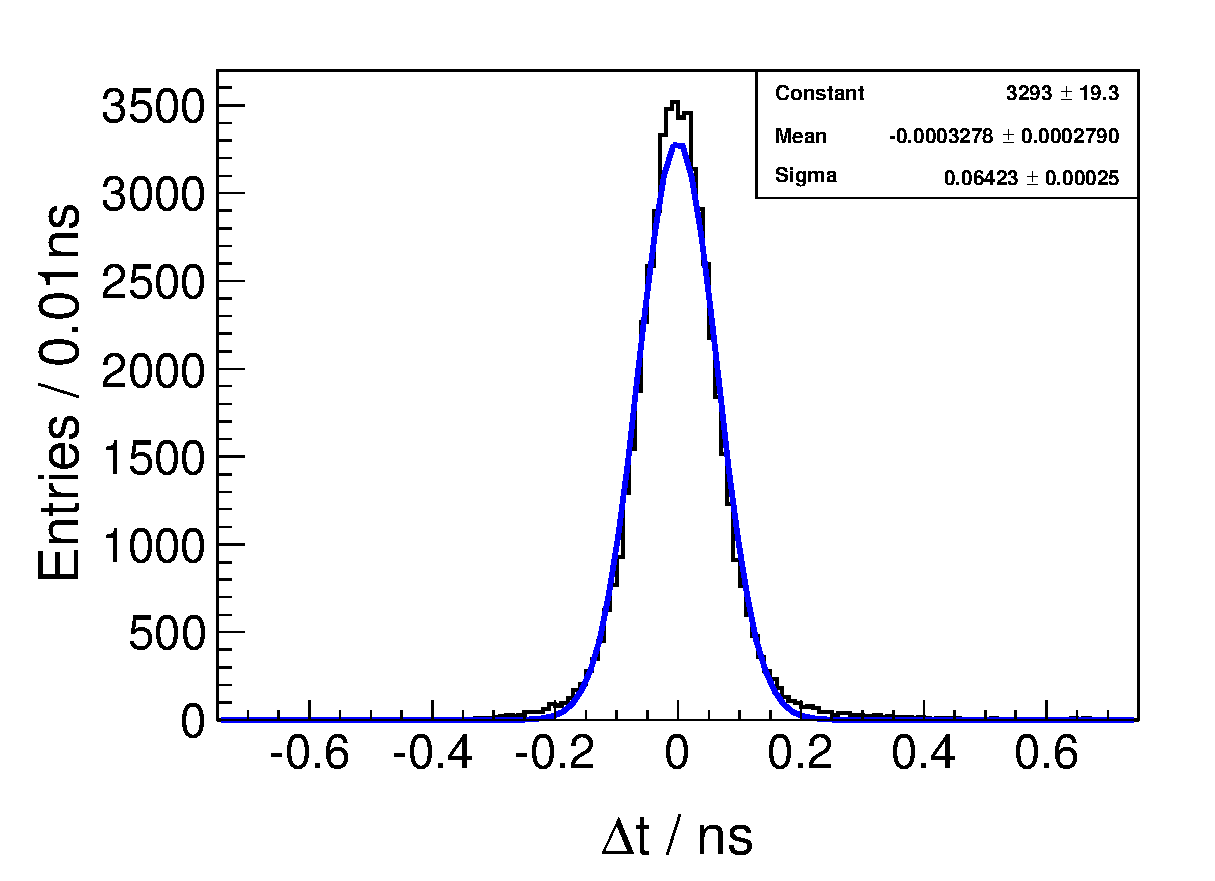
\includegraphics[width=0.9\textwidth]{chap2/resolutiongauss.eps}
\subcaption{时间分辨}
\label{fig:resolutiongauss}
\end{minipage}
\caption{~Z~修正后插值}
\end{figure}

这种对比也说明了先对~Z~进行修正,之后再对~TOT~进行修正是正确的。

\section{小结}

本章利用样条插值方法,从几个不同的方法对~MRPC~的刻度方法进行了研究和分析。根据不同的方法得到的时间分辨,修正完后时间对~Z~,时间对~TOT~的分布等比较,得出对于~BESIII~实验的~MRPC~刻度应该先对~Z~进行修正,然后对~Z~进行修正。
插值方法

%  % !TeX root = ../main.tex
% !TEX root = ../main.tex
% -*- root: ../main.tex -*-
% -*- program: pdflatex -*-
\chapter{构造公式方法}
\section{Z~的修正}
\subsection{Z~向等区间分~bin~}
\subsection{每个~bin~采用~Nov~公式拟合}
\subsection{对得到的~graph~点采用三阶多项式拟合}
\section{TOT~的修正}
\subsection{尝试各种公式}
\subsection{确定这个主项公式}
\section{小结}










  % !TeX root = ../main.tex
% !TEX root = ../main.tex
% -*- root: ../main.tex -*-
% -*- program: pdflatex -*-
\chapter{双端修正}
上两章主要从插值方法和构造公式入手介绍了对TOF的MRPC的离线数据的刻度方法。研究的主要是单端的刻度。这章将介绍双端刻度方法。

\begin{figure}[!h]
\begin{minipage}[!h]{0.5\linewidth}
%\centering
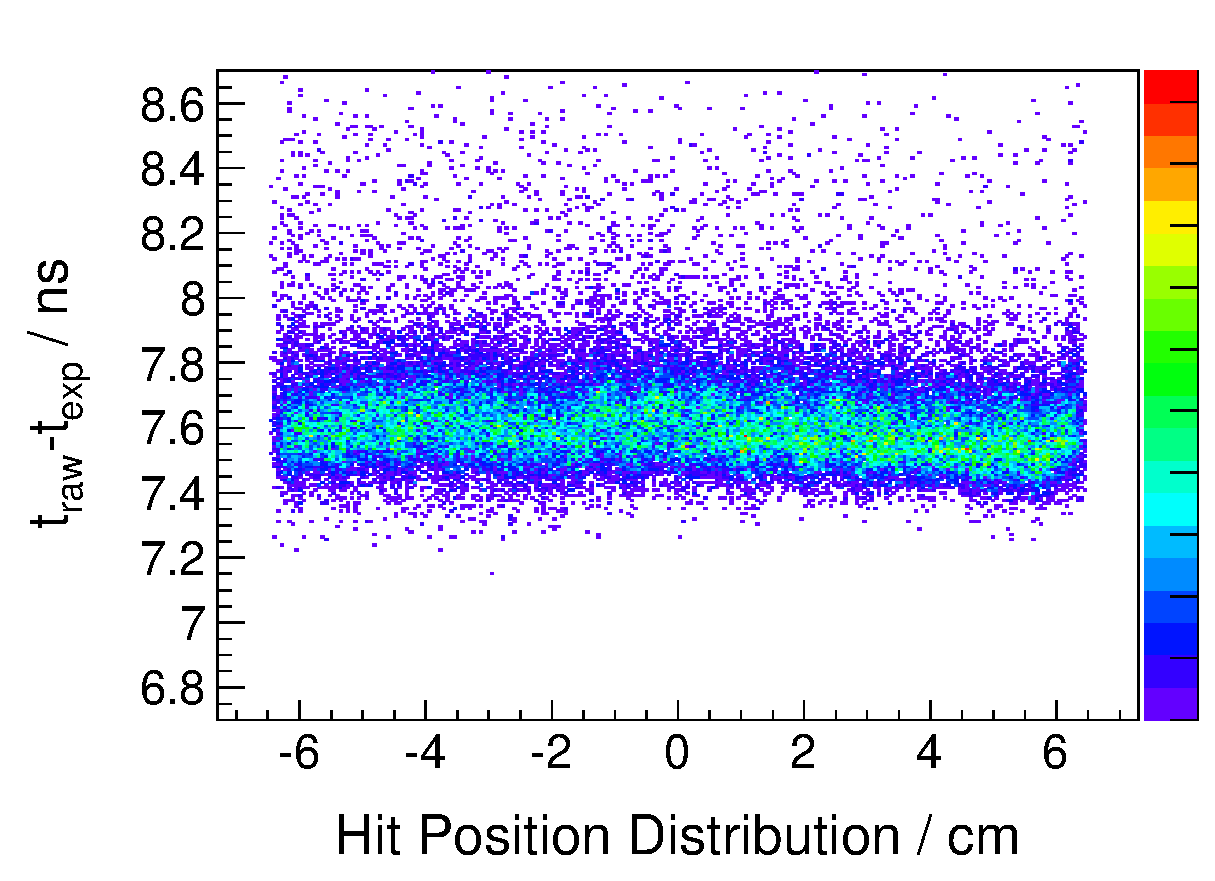
\includegraphics[width=0.9\textwidth]{chap4/combined-tVSz.eps}
\subcaption{双端时间对~Z~的分布}
\label{fig:combined-tVSz}
\end{minipage}%
\hfill
\begin{minipage}[!h]{0.5\linewidth}
%\centering
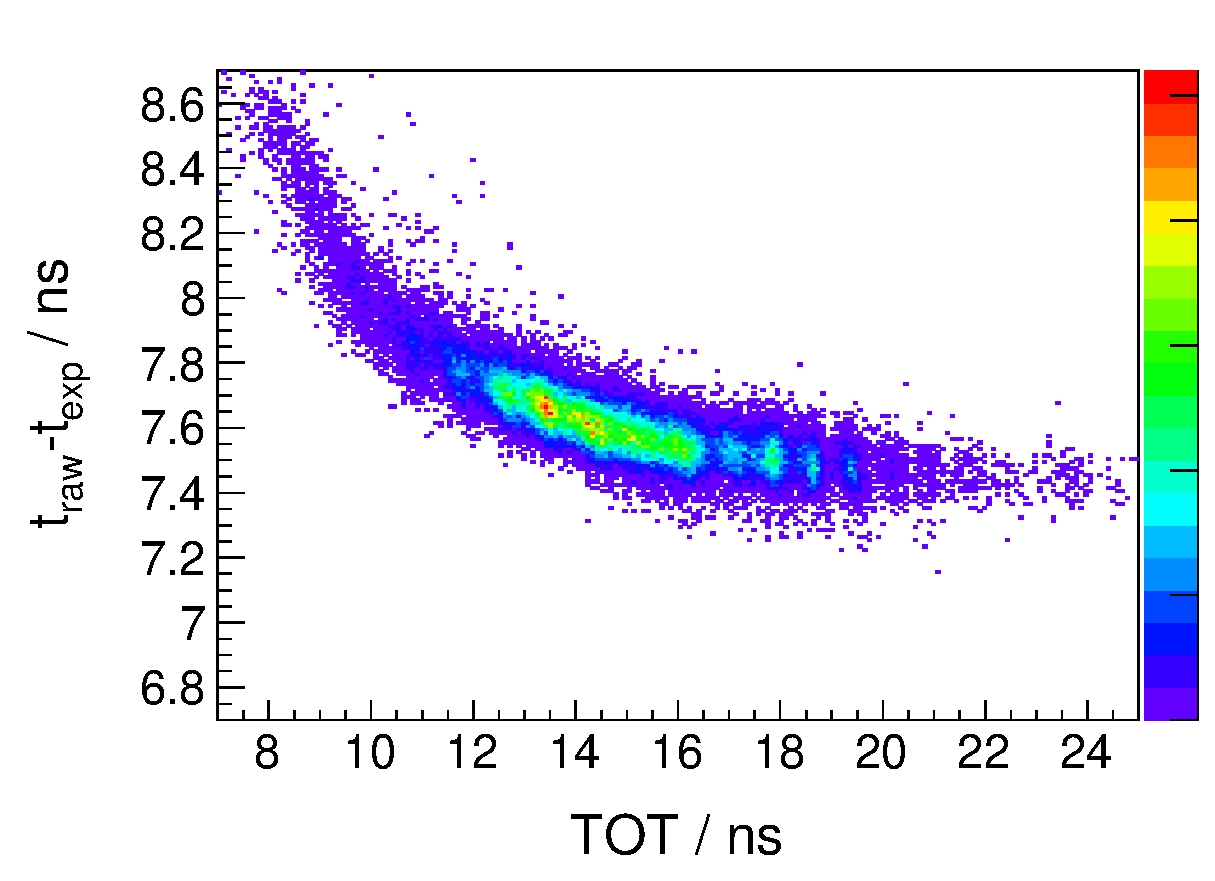
\includegraphics[width=0.9\textwidth]{chap4/combined-tVSq.eps}
\subcaption{时间对~TOT~的分布}
\label{fig:combined-tVSq}
\end{minipage}
\caption{双端时间对~Z~和~TOT~的分布}
\end{figure}

图~\ref{fig:combined-tVSz}~和图~\ref{fig:combined-tVSq}~是双端的时间对~Z~和~TOT~的分布。所谓双端指的是两端时间的平均值,~TOT~采用的也是两端~TOT~的平均值。从图中可以看出,双端的时间对~Z~的依赖很小,主要就是时间对~TOT~的依赖关系。而这时的时间对~TOT~的依赖关系和单端修正~Z~后时间对~TOT~的分布很类似。因此对于双端修正,直接对~TOT~修正,采用和单端修正~Z~后处理时间与~TOT~的关系相同的办法。

\section{双端插值方法}
也是先利用插值方法对双端进行修正。
\section{双端构造公式}
\section{双端对~Z~的修正}
为了绕开径迹外推的信息~zrhit~,采用类似的信息(tleft-tright)/2
\section{小结}













%  \include{chapter/}
%  \include{chapter/}

  % 附录
%  \appendix

  %\include{chapter/chap-req}


%%%%%%%%%%%%%%%%%%%%%%%%%%%%%%
%% 附件部分
%%%%%%%%%%%%%%%%%%%%%%%%%%%%%%
\backmatter

  % 参考文献
  % 使用 BibTeX
  \bibliography{tex}
  \nocite{*}
  % 不使用 BibTeX
  % \include{chapter/bib}

  % 发表文章目录
%  \include{chapter/pub}

  % 个人简历
%  % !TeX root = ../main.tex
% !TEX root = ../main.tex
% -*- root: ../main.tex -*-
% -*- program: pdflatex -*-
\begin{resume}

\begin{resumesection}{基本情况}
郭迎晓,男,河南省新乡市人,1991 年~5 月出生,未婚,
中国科学院高能物理研究所在读硕士研究生。
\end{resumesection}

\begin{resumelist}{教育状况}


2010~年~9~月至~2014~年~6~月,湘潭大学,本科,专业:物理学。

2014~年~9~月至~2017~年~7~月,中国科学院高能物理研究所, 硕士,专业:计算机技术。
\end{resumelist}

\begin{resumelist}{工作经历}
无。
\end{resumelist}

\begin{resumelist}{研究兴趣}
TOF刻度。
\end{resumelist}

\begin{resumelist}{联系方式}
通讯地址:北京市石景山区玉泉路~19~号乙 中国科学院高能物理研究所

邮编:100049

E-mail: guoyingxiao@ihep.ac.cn
\end{resumelist}

\end{resume}


  % 致谢
%  % !TeX root = ../main.tex
% !TEX root = ../main.tex
% -*- root: ../main.tex -*-
% -*- program: pdflatex -*-
\begin{thanks}

三年光景,不过弹指一挥间。前些日子的一个下午在主楼看到那些在四楼大厅焦急等待硕士复试结果的一群学生。不禁回想起自己3年前来所里复试的情景。那时候自己不也和他们一样渴望进入高能所,对未来满怀憧憬。如今,自己也已经完成了自己硕士期间的课题。在此,要对那些曾经在成长路上帮助过我的那些人表示感谢。

首先,需要感谢的是我的导师孙胜森老师。记得和孙老师第一次见面时,他就说年轻人要目标长远,理想远大。孙老师学识渊博,对BESIII探测器软件部分很是了解,更是TOF探测器方面的专家。刚入所时,我对TOF探测器的硬件以及软件都不甚了解,程序也看不懂。在孙老师的帮助下和一次次耐心的讲解下,对BESIII实验的软件有了比较全面的了解,熟悉了TOF探测器的刻度和重建的流程,也能够自己编写一些程序脚本对数据进行处理和检查。在之后对MRPC数据离线刻度方法的研究中更是每次遇到困难都能得到孙老师好的指导和建议。而且孙老师指导学生认真负责,每此的考核报告,都从内容,逻辑,格式,用词等方面对我提出意见。除了在学术上对我的帮助外,孙老师还经常和我聊一些科研工作外的话题,教我一些科研外的东西。临近毕业,我有些迷茫,也对自己有些不满,孙老师也给予了我很大的鼓励和安慰。

然后需要感谢一下林韬师兄。林韬师兄在计算机方面知之甚多,而且很是热心肠。在B406办公室,我和他是邻桌,刚入室的时候,我对编程可谓一窍不通,这个时候林韬时候就经常主动帮助我,教我怎么写结构体和类,教我如何编译。让我慢慢的能够自己写代码,并对程序的运行等等都有了一些了解。他还经常推荐我一些网站和教我一些软件和工具,像github,有道云笔记,IHEPBox等都是他介绍给我并教我如何使用的。我的这些论文的latex模板也是他提供给我的。这里我之所以单独感谢一下林韬师兄是因为大多数情况下,都是他主动帮助我的。这是一个人最难能可贵的品质。

感谢戴忠、于庆洋、董伟伟、付颖、张其安、魏占辰、邴丰、杨佼汪、黎炎等等同学,在怀柔一起去上课,一起去图书馆自习,一起在操场打牌,一起吃串喝酒等等,总之在怀柔有你们这帮同学的陪伴,我有了一个丰富多彩的学习生活。

感谢教育处的保增宽老师,李苏敏老师,陈红珍老师,柯笑晗老师。来所里复试时接待的是你们,感谢你们在包括入学,考核,各类档案以及论文提交等手续给予的帮助。在我打印成绩单需要所里出具证明的时候,在我学生证需要注册的时候,在我对毕业论文的事情有些不清楚询问的时候,每位老师总是很热情。

%尤其需要感谢的是柯笑晗老师,记得中期考核报告第一次提交的那一份中有一个明显的打字错误,于是我把新的版本又一次邮件发给了柯老师,那时候已经是晚上8点50分了,而第二天的早上8:30分就要考核了,我很担心自己的报告来不及更新。而第二天报告的时候,我的报告已经是更新过的。我想,如果报告来不及更新,那个明显的打字错误有很大的可能会对我这次考核的得分有影响。总之,你们对自己的工作认真负责,对学生态度友善。

感谢B406办公室的安芬芬、李新颖、王洪鑫、张坤、周明、方肖、王蒙、肖言佳,马明明、杨荣兴、黄震、张晋、付婷婷、苗楠楠、陆佳达等在学习和生活上对我的帮助和照顾。

感谢父母、弟弟对我学业上的支持。我体质原因,容易上火,每次你们电话都是让我多注意休息,多吃水果。很感谢父母在外打拼,努力赚钱,让我不至于为了家里的生计担忧,能够静下心来好好学习,安心科研。感谢父母在我每次心情不爽的时候可以安慰我,鼓励我。感谢弟弟和他女朋友在16年元旦来看我,给我带礼物,并能够在节假日或者北京天气有变化的时候给我打电话,发短信。你们永远是我最坚强的后盾。


\end{thanks}
















\end{document}
